\documentclass[10pt,a4paper]{article}
\usepackage{fullpage}
\usepackage{graphicx}
\usepackage{fancyhdr}
\setlength{\headheight}{13pt}
\pagestyle{fancy}

% default sans-serif
\renewcommand{\familydefault}{\sfdefault}

% no lines for headers and footers
\renewcommand{\headrulewidth}{0pt}
\renewcommand{\footrulewidth}{0pt}

% header
\fancyhf{}
\lhead{GWD-R}
\rhead{\today}

% footer
\lfoot{occi-wg@ogf.org}
\rfoot{\thepage}

% paragraphs need some space...
\setlength{\parindent}{0pt}
\setlength{\parskip}{1ex plus 0.5ex minus 0.2ex}

% some space between header and text...
\headsep 13pt

\setcounter{secnumdepth}{4}

\begin{document}

% header on first page is different
\thispagestyle{empty}

GWD-R \hfill  Thijs Metsch, Platform Computing\\
OCCI-WG \hfill  Andy Edmonds, Intel\\
\rightline {October 7, 2010}\\
\rightline {Updated: \today}

\vspace*{0.5in}

\begin{Large}
\textbf{Open Cloud Computing Interface - Infrastructure}
\end{Large}

\vspace*{0.5in}

\underline{Status of this Document}

This document provides information to the community regarding the specification of the Open Cloud Computing Interface. Distribution is unlimited.

\underline{Obsoletes}

This document obsoletes GFD-xxx [REFERENCE].

\underline{Copyright Notice}

Copyright \copyright Open Grid Forum (2009-2010). All Rights Reserved.

\underline{Trademarks}

OCCI is a trademark of the Open Grid Forum.

\underline{Abstract}

This document, part of a document series, produced by the OCCI working group within the Open Grid Forum (OGF), provides a high-level definition of a Protocol and API. The document is based upon previously gathered requirements and focuses on the scope of important capabilities required to support modern service offerings. 

\newpage
\tableofcontents
\newpage

\section{Introduction}

The Open Cloud Computing Interface (OCCI) is a RESTful Protocol (and API) for all kinds of Management tasks. Originally initiated to create a remote management API for IaaS model based Services, allowing for the development of interoperable tools for common tasks including deployment, autonomic scaling and monitoring, it now can be used to severe other models as well. To be modular and extensible the current specification itself is currently split into three complimentary documents:

\begin{itemize}
\item Core - this defines the OCCI model
\item HTTP Rendering - this defines how to manipulate the core model using the OCCI RESTful API. The document defines how the OCCI model can be communicated and thus serialized using HTTP.
\item Infrastructure - this defines the infrastructure domain resource types, the required attributes for each and the actions that can be taken on each.
\end{itemize}

\section{Notational Conventions}

All these parts and the information within are mandatory for implementors (unless otherwise specified). The key words "MUST", "MUST NOT", "REQUIRED", "SHALL", "SHALL NOT", "SHOULD", "SHOULD NOT", "RECOMMENDED", "MAY", and "OPTIONAL" in this document are to be interpreted as described in RFC 2119. 

UML activity diagrams do not specify how OCCI should be rendered but what possible request and outcomes can be.

% begin infrastructure content

\section{Infrastructure}

The infrastructure domain resource types within OCCI, including their specification definitions, are:
\begin{itemize}
\item Compute: Information processing resources.
\item Network: Interconnection resources.
\item Storage: Information recording resources.
\end{itemize}
These infrastructure resource types inherit Resource base type and all its attributes. OCCI implementors MUST implement these. The HTTP Rendering document define how to interact with these resource types using RESTful communication. OCCI makes an ideal interoperable boundary interface between the web and the internal resource management system of infrastructure providers.

As REQUIRED by the OCCI Core specification every resource type instantiated that is a subclass of Resource MUST be assigned a Category that identifies the instantiated resource type. Each such Category MUST be related to the Resource base type Category. These Categories, the core categories, MUST always remain immutable to any client.

The following table describe the Category defined for each of the infrastructure Resource subtypes:

\begin{tabular}{llllll}
Term&Scheme&Title&Attribute&Actions&Related-Category\\
\hline
compute & http://schemas.ogf.org/occi/infrastructure\# & Compute Resource & See Below & See Below & http://schemas.ogf.org/occi/core\#resource\\
storage & http://schemas.ogf.org/occi/infrastructure\# & Storage Resource & See Below & See Below & http://schemas.ogf.org/occi/core\#resource\\
network & http://schemas.ogf.org/occi/infrastructure\# & Network Resource & See Below & See Below & http://schemas.ogf.org/occi/core\#resource\\
\end{tabular}

The following sections on Compute, Storage and Network detail the Attributes and Actions defined for each resource type.

\subsection{Compute}
The Compute Resource type is assigned the http://schemas.ogf.org/occi/infrastructure\#compute Category. A Compute Resource instance MUST at least expose this Category.

\subsubsection{Attributes}
The attributes that MUST be exposed by an instance of the Compute Resource type are as follows:

\begin{tabular}{lllll}
Attribute&Type&Multiplicity&Client Access&Description\\
\hline
occi.compute.architecture & String Enumeration, \{x86, x64\} & 1 & read-many/write-many & CPU Architecture of the instance.\\
occi.compute.cores & Integer & 1 & read-many/write-many & Number of CPU cores assigned to the instance.\\
occi.compute.hostname & String & 1 & read-many/write-many & Fully Qualified DNS hostname for the instance.\\
occi.compute.speed & Float, ${\mathbf 10}^9$ (giga) & 1 & read-many/write-many & CPU Clock frequency (speed) in gigahertz.\\
occi.compute.memory & Float, ${\mathbf 10}^9$ (giga) & 1 & read-many/write-many & Maximum RAM in gigabytes allocated to the instance.\\
occi.compute.state & Enumeration, \{active, inactive, suspended\} & 1 & read-only & Current state of the instance.\\
\end{tabular}

\subsubsection{Actions}
Actions can be performed upon instances of the Compute Resource type. The set that MUST be supported are as follows:

\begin{tabular}{lll}
Action&Target State&Parameters\\
\hline
http://schemas.ogf.org/occi/infrastructure/compute/action\#start & active & None\\
http://schemas.ogf.org/occi/infrastructure/compute/action\#stop & inactive & String Enumeration \{graceful, acpioff, poweroff\}\\
http://schemas.ogf.org/occi/infrastructure/compute/action\#restart & active (via stop and start chain) & String Enumeration {graceful, warm, cold}\\
http://schemas.ogf.org/occi/infrastructure/compute/action\#suspend & suspended & String Enumeration {hibernate, suspend }\\
\end{tabular}

\subsubsection{States}
Below illustrates the state diagram based on the actions defined above in REF.

%\clearpage
\begin{figure}[!h]
	\centering
	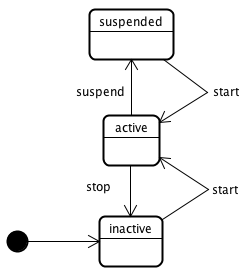
\includegraphics[scale=0.4]{dia/compute-state.png}
	\caption{State diagram for Compute}
	\label{fig:compute_state}
\end{figure}

\subsection{Network}
The Network Resource type is assigned the http://schemas.ogf.org/occi/infrastructure\#network Category. A Network Resource instance MUST at least expose this Category.

\subsubsection{Attributes}
The attributes that MUST be exposed by an instance of the Network Resource type are as follows:

\begin{tabular}{lllll}
Attribute&Type&Multiplicity&Client Access&Description\\
\hline
occi.network.vlan & Integer, 0-4095 & 0..1 & read-many/write-many & 802.1q VLAN Ientifier (e.g. 4095).\\
occi.network.label & Token & 0..1 & read-many/write-many & Tag based VLANs (e.g. external-dmz).\\
occi.network.address & IPv4 or IPv6 Address, CIDR notation & 1..* & read-many/write-many & Internet Protocol(IP) network address (e.g. 192.168.0.1/24, fc00::/7)\\
occi.network.gateway & IPv4 or IPv6 Address & 0..1 & read-many/write-many & Internet Protocol(IP) network address (e.g. 192.168.0.1/24, fc00::/7)\\
occi.network.allocation & String Enumeration, {auto, dhcp, manual} & 1 & read-many/write-many & Address mechanism: auto use the provider default policy dhcp use the dynamic host configuration protocol manual use user supplied static network configurations.\\
occi.network.state & Enumeration, {active, inactive} & 1 & read-only & Current state of the instance.\\
\end{tabular}

\subsubsection{Actions}
Actions can be performed upon instances of the Network Resource type. The set that must be supported are as follows:

\begin{tabular}{lll}
Action&Target State&Parameters\\
\hline
http://schemas.ogf.org/occi/infrastructure/compute/action\#up & active & None\\
http://schemas.ogf.org/occi/infrastructure/compute/action\#down & inactive & None\\
\end{tabular}

\subsubsection{States}
Below illustrates the state diagram based on the actions defined above in REF.

%\clearpage
\begin{figure}[!h]
	\centering
	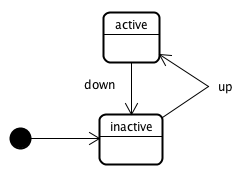
\includegraphics[scale=0.4]{dia/network-state.png}
	\caption{State diagram for Network}
	\label{fig:network_state}
\end{figure}

\subsection{Storage}
The Storage Resource type is assigned the http://schemas.ogf.org/occi/infrastructure\#storage Category. A Storage Resource instance MUST at least expose this Category.

\subsubsection{Attributes}
The attributes that MUST be exposed by an instance of the Storage Resource type are as follows:

\begin{tabular}{lllll}
Attribute&Type&Multiplicity&Client Access&Description\\
\hline
occi.storage.size & Float, ${\mathbf 10}^9$ (giga) & 1 & read-many/write-many & Storage size in gigabytes of the instance.\\
occi.storage.state & String Enumeration, \{online, offline, degraded\} & 1 & read-only & Current status of the instance.\\
value & value & value & value & value\\
\end{tabular}

\subsubsection{Actions}
Actions can be performed upon instances of the Storage Resource type. The set that MUST be supported are as follows:

\begin{tabular}{lll}
Action&Target State&Parameters\\
\hline
http://schemas.ogf.org/occi/infrastructure/storage/action\#online & online & None\\
http://schemas.ogf.org/occi/infrastructure/storage/action\#offline & offline & None\\
http://schemas.ogf.org/occi/infrastructure/storage/action\#backup & None & None\\
http://schemas.ogf.org/occi/infrastructure/storage/action\#snapshot & None & None\\
http://schemas.ogf.org/occi/infrastructure/storage/action\#resize & None & size Float  ${\mathbf 10}^9$\\
\end{tabular}

\subsubsection{States}
Below illustrates the state diagram based on the actions defined above in 4.3.2.

%\clearpage
\begin{figure}[!h]
	\centering
	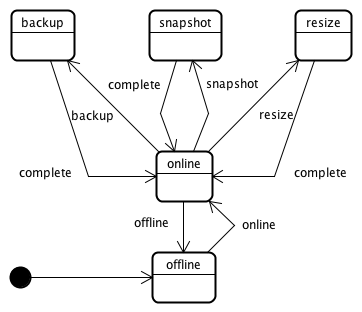
\includegraphics[scale=0.4]{dia/storage-state.png}
	\caption{State diagram for Storage}
	\label{fig:storage_state}
\end{figure}

% end infrastructure content

\section{Contributors}

Editors: Andy Edmonds, Thijs Metsch \\
Contributors: Alexander Papaspyrou, Ralf Nyren, Sam Johnston

\textbf{TBD: Bunch op people missing here - create table\ldots}

\section{Appendix}

\subsection{Examples for rendering the OCCI model in the HTTP Header}

\begin{verbatim}

\end{verbatim}

\section{Glossary}

\begin{tabular}{l|l}
Term & Description \\
\hline
OCCI & Open Cloud Computing Interface \\
URN & Unified Resource Name \\
URL & TBD \\
URI & TBD \\
\end{tabular}

\section{Intellectual Property Statement}

The OGF takes no position regarding the validity or scope of any intellectual property or other rights that might be claimed to pertain to the implementation or use of the technology described in this document or the extent to which any license under such rights might or might not be available; neither does it represent that it has made any effort to identify any such rights. Copies of claims of rights made available for publication and any assurances of licenses to be made available, or the result of an attempt made to obtain a general license or permission for the use of such proprietary rights by implementers or users of this specification can be obtained from the OGF Secretariat.

The OGF invites any interested party to bring to its attention any copyrights, patents or patent applications, or other proprietary rights which may cover technology that may be required to practice this recommendation. Please address the information to the OGF Executive Director.

\section{Disclaimer}

This document and the information contained herein is provided on an ''As Is'' basis and the OGF disclaims all warranties, express or implied, including but not limited to any warranty that the use of the information herein will not infringe any rights or any implied warranties of merchantability or fitness for a particular purpose.

\section{Full Copyright Notice}

Copyright \copyright Open Grid Forum (2009-2010). All Rights Reserved.

This document and translations of it may be copied and furnished to others, and derivative works that comment on or otherwise explain it or assist in its implementation may be prepared, copied, published and distributed, in whole or in part, without restriction of any kind, provided that the above copyright notice and this paragraph are included on all such copies and derivative works. However, this document itself may not be modified in any way, such as by removing the copyright notice or references to the OGF or other organizations, except as needed for the purpose of developing Grid Recommendations in which case the procedures for copyrights defined in the OGF Document process must be followed, or as required to translate it into languages other than English.

The limited permissions granted above are perpetual and will not be revoked by the OGF or its successors or assignees.

\section{References}

Note that only permanent documents should be cited as references. Other items, such as Web pages or working groups, should be cited inline (i.e., see the Open Grid Forum, http://www.ogf.org). References should conform to a standard such as used by IEEE/ACM, MLA, Chicago or similar. Include an author, year, title, publisher, place of publication. For online materials, also add a URL. It is acceptable to separate out ''normative references,'' as IETF documents typically do. Some sample citations: 

\end{document}
